\newpage

\section{Экспериментальные данные}

Эксперимент проводится для данных курса акций YNDX.

Задается временной ряд 
$$x_{1}, x_{2}, x_{3}, ..., x_{N}, \quad x_{i} \in \mathbb{R}^{5}$$
$$
    x_{i} = 
    \begin{bmatrix}
        c_{i} & o_{i} & h_{i} & l_{i} & a_{i}
    \end{bmatrix}^{T},
$$
где \\
$c_{i}$ - цена закрытия, \\
$o_{i}$ - цена открытия, \\
$h_{i}$ - максимальная цена, \\
$l_{i}$ - минимальная цена, \\
$a_{i}$ - ответ модели автоследования ($a_{i} = 0$ в базовом варианте обучения модели)

\subsection{Стационарность}

Исходный ряд приводится к стационарному виду следующими преобразованиями: \\
1) Дифференцирование: $y'_{t} = y_{t} - y_{t-1}$ \\ 
2) Сезонное дифференцирование $y''_{t} = y'_{t} - y'_{t-s}, \ s=5$ \\

Т.к. торги открыты только в будние дни, то выбранная длина сезона $s=5$.

\begin{figure}[h!t]\center
\subfloat[]
{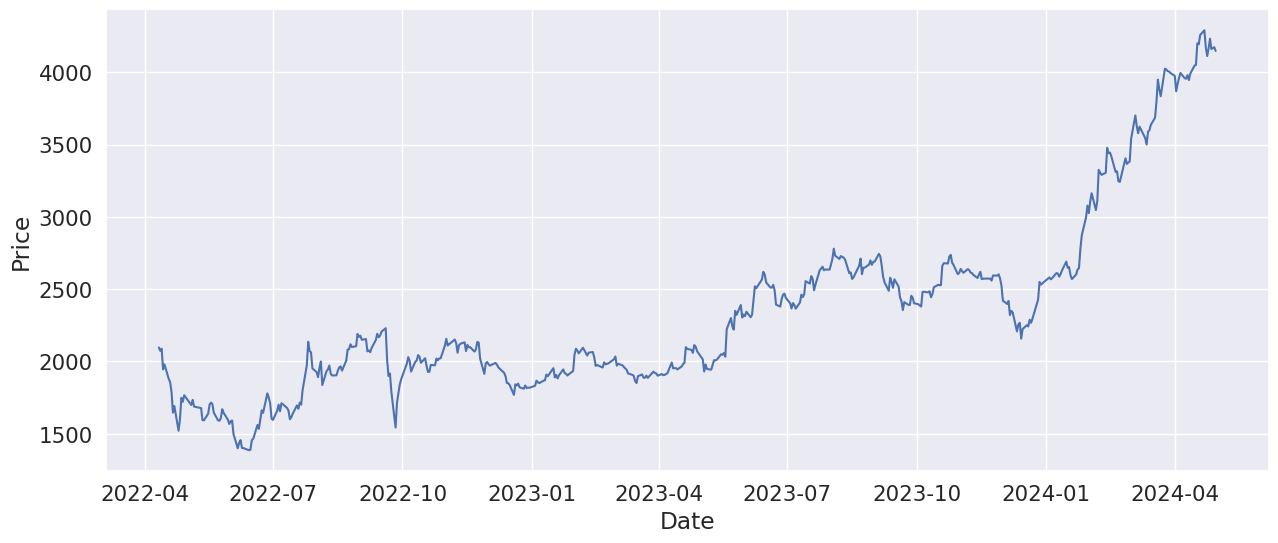
\includegraphics[width=0.5\textwidth]{results/yndx.png}}
\subfloat[]
{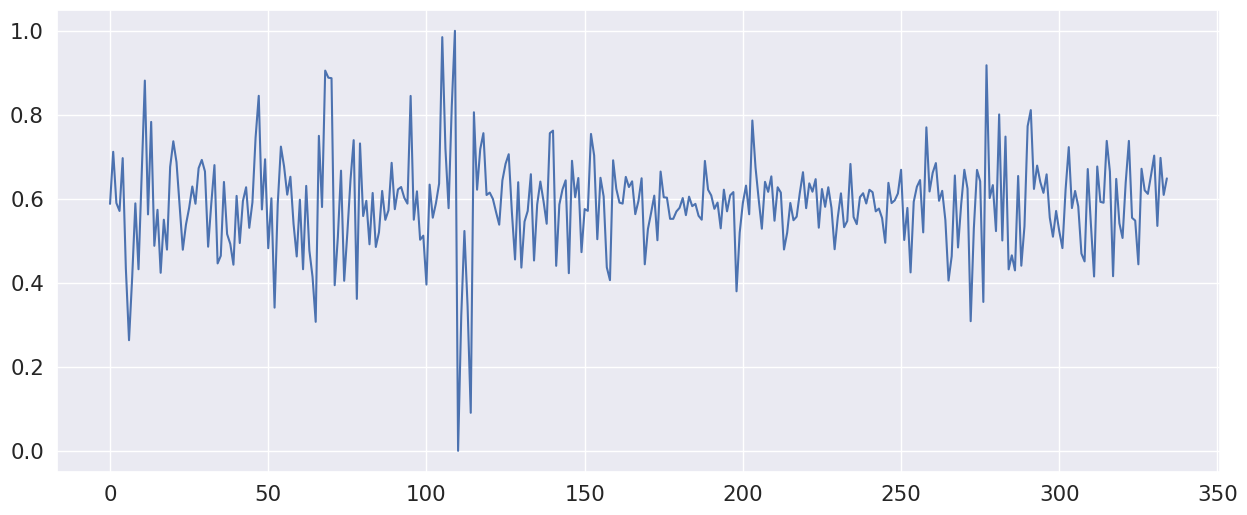
\includegraphics[width=0.5\textwidth]{results/yndx_stationary.png}}
\caption{Временной ряд курса акций YNDX до и после преобразований}
\end{figure}

Для проверки ряда на стационарность используется критерий KPSS~\cite{Критерии стационарности 1, Критерии стационарности 2}: \\
Для полученного ряда $p-value > 0.01$ \\
Для исходного ряда $p-value < 0.01$ 

Для визуальной оценки стационарности ряда также построим Q-Q plot:

\begin{figure}[h!t]\center
{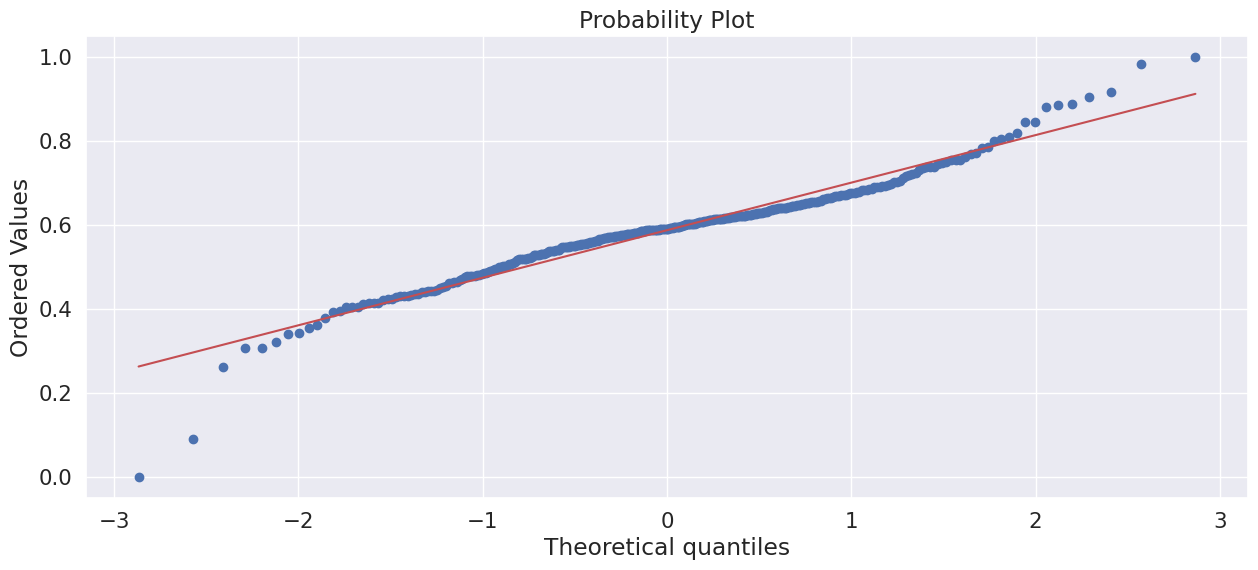
\includegraphics[width=0.8\textwidth]{results/qqplot.png}}
\caption{Q-Q plot полученного ряда}
\end{figure}

Видно, что точки на графике примерно лежат на прямой линии, следовательно распределение полученного временного ряда близко к нормальному.

Также воспользуемся анализом автокорреляционной функции:

\begin{figure}[h!t]\center
{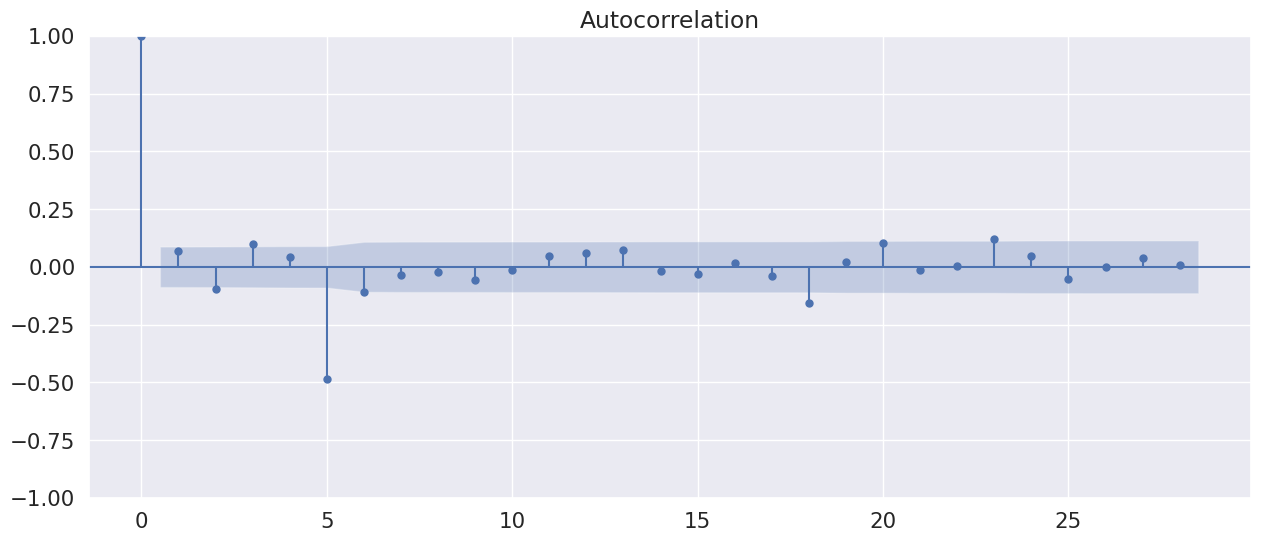
\includegraphics[width=0.8\textwidth]{results/acf.png}}
\caption{ACF полученного ряда}
\end{figure}

Близкие к нулю значения автокорреляций также указывают на стационарность полученного ряда.

\subsection{Составление выборки}

Методом скользящего окна составляется выборка $\mathfrak{D}=(\mathbf{X},\mathbf{Y})$:

\begin{figure}[h!t]\center
{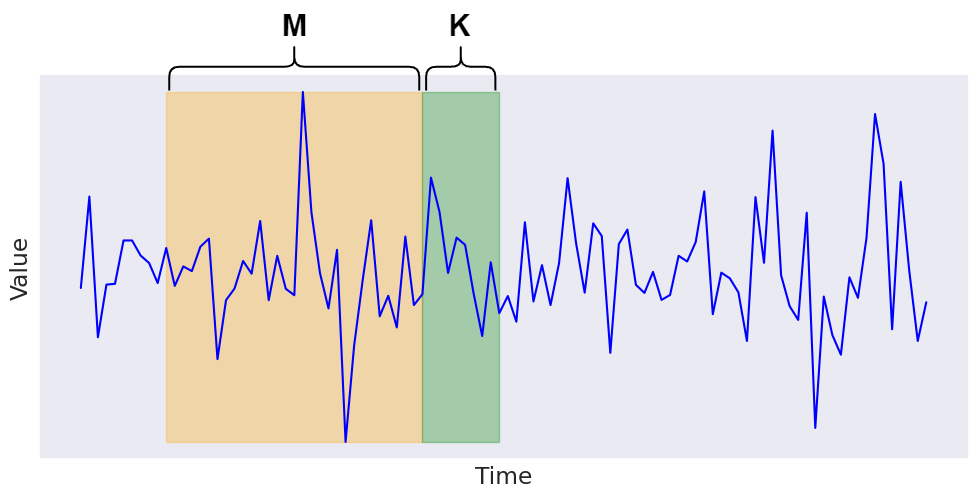
\includegraphics[width=0.8\textwidth]{results/slidingwindow.png}}
\caption{Метод скользящего окна}
\end{figure}

\small
\[
\mathbf{X} = 
\begin{pmatrix}
x_{1} & x_{2} & ... & x_{M}\\
x_{2} & x_{3} & ... & x_{M+1} \\
x_{3} & x_{4} & ... & x_{M+2} \\
\vdots & \vdots & \vdots & \vdots \\
x_{N-K-M+1} & x_{N-K-M+2} & ... & x_{N-K} \\
\end{pmatrix},
\mathbf{Y} = \begin{pmatrix}
c_{M+1} & c_{M+2} & ... & c_{M+K}\\
c_{M+2} & c_{M+3} & ... & c_{M+K+1} \\
c_{M+3} & c_{M+4} & ... & c_{M+K+2} \\
\vdots & \vdots & \vdots & \vdots \\
c_{N-K+1} & c_{N-K+2} & ... & c_{N} \\
\end{pmatrix},
\]
\normalsize

где  $M$ - размер окна, $K$ - горизонт прогнозирования.

\bigskip

В качестве целевых значений используется цена закрытия.

\bigskip

В соотношении 80/20 выборка делится на обучающую и тестовую части: YNDX-train, YNDX-test.